% !TEX encoding = UTF-8 Unicode
% !TEX root = SystemTemplate.tex

\documentclass{book}
% !TEX root = SystemTemplate.tex

\usepackage[width=6.5in, height=9.2in, top=1.0in, papersize={8.5in,11in}]{geometry}
\usepackage[pdftex]{graphicx}
%\usepackage{draftwatermark}
\usepackage{amsmath}
\usepackage{amsthm}
\usepackage{amssymb}
%\usepackage{txfonts}
\usepackage{textcomp}
%\usepackage{amsthm}

\usepackage[all]{xy}
\usepackage{fancyhdr}
\pagestyle{fancy}
\usepackage{hyperref}
\usepackage{verbatim}
\usepackage{algorithm}
\usepackage{algorithmic}
\usepackage{array}
\usepackage{color}
\usepackage{listings}
\lstset{language=c,frame=ltrb,framesep=5pt,basicstyle=\normalsize,
 keywordstyle=\ttfamily\color{DarkRed},
identifierstyle=\ttfamily\color{DarkBlue}\bfseries,
commentstyle=\color{OliveGreen},
stringstyle=\ttfamily,
showstringspaces=false,tabsize = 3}
\usepackage{calc}
\usepackage{doxygen}
\usepackage[utf8]{inputenc}
\usepackage{makeidx}
\usepackage{multicol}
\usepackage{multirow}
\usepackage[table]{xcolor}

\definecolor{color02}{rgb}{0.18,0.35,0.59}
\definecolor{color03}{rgb}{0.44,0.59,0.82}
\definecolor{color06}{rgb}{0.35,0.35,0.35}


\newtheorem{summary}{Summary:}
\newtheorem{example}{Example:}


\definecolor{OliveGreen}{cmyk}{0.64,0,0.95,0.40}
\definecolor{DarkBlue}{cmyk}{0.76,0.76,0,0.20}
\definecolor{DarkRed}{cmyk}{0,1,1,0.45}


\def      \RR             {{\mathbb R}} 
\def      \DS            {\displaystyle} 

\setlength{\oddsidemargin}{0mm} 
\setlength{\evensidemargin}{0mm} 

%\SetWatermarkLightness{0.975}
%\SetWatermarkScale{6}
%\SetWatermarkText{\includegraphics{test.png}}

\pagestyle{fancy}
\renewcommand{\chaptermark}[1]{\markboth{#1}{}}
\renewcommand{\sectionmark}[1]{\markright{\thesection\ #1}}
\fancyhf{}
\fancyhead[LE,RO]{\bfseries\thepage}
\fancyhead[LO]{\bfseries\rightmark}
\fancyhead[RE]{\bfseries\leftmark}
\fancyfoot[LE,RO]{Confidential and Proprietary}
%\renewcommand{\headrulewidth}{0.5pt}
%\renewcommand{\footrulewidth}{0pt}
%\addtolength{\headheight}{0.5pt}
%\setlength{\footskip}{0mm}
%\renewcommand{\footruleskip}{0pt}


\definecolor{MSBlue}{rgb}{.204,.353,.541}
\definecolor{MSLightBlue}{rgb}{.31,.506,.741}
\definecolor{MSBlue1}{rgb}{0.18,0.35,0.59}
\definecolor{MSBlue2}{rgb}{0.44,0.59,0.82}
\definecolor{MSBlue3}{rgb}{0.35,0.35,0.35}


\usepackage{titlesec}
\titleformat{\chapter}[display]
{\normalfont\bfseries\color{MSBlue1}}    %\normalfont\bfseries\filcenter}
{\LARGE\thechapter}
{1ex}
{\titlerule[2pt]
\vspace{2ex}%
\LARGE}
[\vspace{1ex}%
{\titlerule[2pt]}]

\definecolor{MSBlue}{rgb}{.204,.353,.541}
\definecolor{MSLightBlue}{rgb}{.31,.506,.741}
\definecolor{MSBlue1}{rgb}{0.18,0.35,0.59}
\definecolor{MSBlue2}{rgb}{0.44,0.59,0.82}
\definecolor{MSBlue3}{rgb}{0.35,0.35,0.35}

%\titleformat*{\section}{\Large\bfseries\sffamily\color{MSBlue}}
%\titleformat*{\subsection}{\large\bfseries\sffamily\color{MSLightBlue}}
%\titleformat*{\section}{\Large\bfseries\color{MSBlue1}}
%\titleformat*{\subsection}{\large\bfseries\color{MSBlue2}}

\titleformat*{\section}{\Large\bfseries\color{MSBlue}}
\titleformat*{\subsection}{\large\bfseries\color{MSLightBlue}}
\titleformat*{\subsubsection}{\large\bfseries\color{MSBlue3}}
\setcounter{secnumdepth}{3}
\renewcommand{\thesubsubsection}{\thesubsection.\alph{subsubsection}}

 % This sets the format.

% Add your title page contents here 
\title{{\color{MSBlue1} \rule{\linewidth}{0.5mm}}\\[2mm] {\huge \bfseries \color{MSBlue1} Product Title }\\[-1mm] {\color{MSBlue1}\rule{\linewidth}{0.5mm}} \\  \vfill
{\LARGE \bfseries \color{MSBlue2} Senior Design Final Documentation }\\  \vfill 
{\color{MSBlue1} The Software Engineering Adventure Line} }
\author{\color{MSBlue1}  Jonathan Tomes \and \color{MSBlue1} Erik Hattervig \and  \color{MSBlue1} Andrew Koc }
\date{\color{MSBlue1} \today}


\begin{document}
\frontmatter
\maketitle


\tableofcontents
\listoffigures
\listoftables
\listofalgorithms


% !TEX root = SystemTemplate.tex

\chapter{Mission}

Mission statement inserted here.  % add mission statement to mission.tex
% !TEX root = SystemTemplate.tex

\chapter{Document Preparation and Updates}

Current Version [X.X.X]
\vspace*{5mm}

{\color{MSBlue3}
\noindent
\textit{Prepared By:}\\
\textit{Team Member \#1}\\
\textit{Team Member \#2}\\
\textit{Team Member \#3}
}

\vfill
\noindent
{\color{color02} \textit{\textbf{Revision History}}}\\
\begin{tabular}{|>{\raggedright}p{1.5cm}|>{\raggedright}p{3cm}|>{\raggedright}p{1.5cm}|>{\raggedright}p{9cm}|}
\hline
\textit{\textbf{Date}} &  \textit{\textbf{Author}} & \textit{\textbf{Version}} & \textit{\textbf{Comments}}\tabularnewline
\hline
 \textit{\textbf{2/2/12}} & \textit{Team Member \#1} & \textit{1.0.0} & \textit{Initial version}\tabularnewline
\hline
\textit{\textbf{3/4/12}} & \textit{Team Member \#3} & \textit{1.1.0} & \textit{Edited version}\tabularnewline
\hline
 &  &  & \tabularnewline
 \hline
 &  &  & \tabularnewline
\hline
 &  &  & \tabularnewline
\hline
 &  &  & \tabularnewline
\hline
 &  &  & \tabularnewline
\hline
\end{tabular}
\vfill



 
\mainmatter

%%  Add to the following chapters

% !TEX root = SystemTemplate.tex

\chapter{Overview and concept of operations}

The overview should take the form of an executive summary.  Give the reader a feel 
for the purpose of the document, what is contained in the document, and an idea 
of the purpose for the system or product. 


\section{Scope}
What scope does this document cover? 


\section{Purpose}
What is the purpose of the system or product? 


\subsection{Major System Component \#1}
Describe briefly the role this major component plays in this system. 

\subsection{Major System Component \#2}
Describe briefly the role this major component plays in this system. 

\subsection{Major System Component \#3}
Describe briefly the role this major component plays in this system. 

\section{Systems Goals}
Briefly describe the overall goals this system plans to achieve.  These goals are 
typically provided by the stakeholders.  This is not intended to be a detailed 
requirements listing.  Keep in mind that this section is still part of the Overview. 

\section{System Overview and Diagram}
Provide a more detailed description of the major system components without getting 
too detailed.  This section should contain a high-level block and/or flow diagram 
of the system highlighting the major components.   See Figure~\ref{systemdiagram}.    This is a floating figure environment.  \LaTeX\ will try to put it close to where it was typeset but will not allow the figure to be split if moving it can not happen.   Figures, tables, algorithms and many other floating environments are automatically numbered and placed in the appropriate type of table of contents.  You can move these and the numbers will update correctly.

\begin{figure}[tbh]
\begin{center}
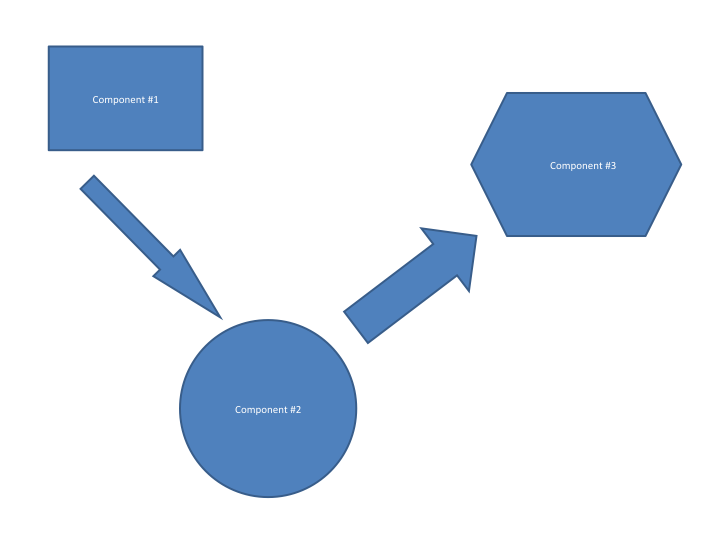
\includegraphics[width=0.75\textwidth]{./diagram}
\end{center}
\caption{A sample figure .... System Diagram \label{systemdiagram}}
\end{figure}

\section{Technologies Overview}
This section should contain a list of specific technologies used to develop the 
system.  The list should contain the name of the technology, brief description, 
link to reference material for further understanding, and briefly how/where/why 
it was used in the system.    See Table~\ref{somenumbers}.  This is a floating table environment.  \LaTeX\ will try to put it close to where it was typeset but will not allow the table to be split.   
\begin{table}[tbh]
\begin{center}
\begin{tabular}{|r|l|}
  \hline
  7C0 & hexadecimal \\
  3700 & octal \\ \cline{2-2}
  11111000000 & binary \\
  \hline \hline
  1984 & decimal \\
  \hline
\end{tabular}
\caption{A sample Table ... some numbers. \label{somenumbers}}
\end{center}
\end{table}


% !TEX root = SystemTemplate.tex


\chapter{Project Overview}
This section provides some housekeeping type of information with regard to the 
team, project, etc. 



\section{Team Members and Roles}
The team consists of Erik Hattervig, Andrew Koc, and Jonathon Tomes. Erik Hattervig is the Product Owner, Andrew Koc is the Technical Lead, and Jonathon Tomes is the Scrum Master. Erik is responsible for understanding the overall expectations of the product and communication with the customer about specific details regarding the operation and design of the product. Andrew is responsible for designing the technical aspects of the code. Jonathon is responsible for managing meetings and communication between team members and making sure the project is on schedule.


\section{Project  Management Approach}
%This section will provide an explanation of the basic approach to managing the 
%project.  Typically, this would detail how the project will be managed through 
%a given Agile methodology.  The sprint length (i.e. 2 weeks) and product backlog 
%ownership and location (ex. Trello) are examples of what will be discussed.  An 
%overview of the system used to track sprint tasks, bug or trouble tickets, and 
%user stories would be warranted.

	The sprint length for this project was 2 weeks. We began with a meeting to
decide the user needs and split the program accordingly. Each of us would code
different parts of the program and then we would all test and re-code as needed.

	The code was stored, backed up, and shared through git hub. The back log and ownership 
was tracked through Trello. The user stories were condensed and placed on Trello to help 
design break points to split up the program between team members. 

\section{Phase  Overview}
%If the system will be implemented in phases, describe those phases/sub-phases (design, 
%implementation, testing, delivery) and the various milestones in this section. 
 %This section should also contain a correlation between the phases of development 
%and the associated versioning of the system, i.e. major version, minor version, 
%revision. 

The first phase of this Testing program was just to begin working on the program.
The main purpose was to get to receive a root directory, find a .cpp file
in the root. It would then write a log file that starting with a time stamp to
be used later to record the results of tests.
	
	After that it would a crawl through the sub directories recursively
starting at the root, looking for .tst files that would be test cases for 
the program. Along with these would be .ans files that would allow us to
compare the program output and see wich test cases failed. 
	
	It would then out put the results of each test to a log file. With a final
log write that writes the percentage of passed and failed tests.

\section{Terminology and Acronyms}
%Provide a list of terms used in the document that warrant definition.  Consider 
%industry or domain specific terms and acronyms as well as system specific.
none. 

% !TEX root = SystemTemplate.tex
\chapter{User Stories, Backlog and Requirements}
\section{Overview}


The overview should take the form of an executive summary.  Give the reader a feel 
for the purpose of the document, what is contained in the document, and an idea 
of the purpose for the system or product. 

 The userstories 
are provided by the stakeholders.  You will create he backlogs and the requirements, and document here.  
This chapter should contain 
details about each of the requirements and how the requirements are or will be 
satisfied in the design and implementation of the system.

Below:   list, describe, and define the requirements in this chapter.  
There could be any number of sub-sections to help provide the necessary level of 
detail. 





\subsection{Scope}
This document covers our basic user stories and requirements for this program.

% What scope does this document cover?  This document would contain stakeholder information, 
% initial user stories, requirements, proof of concept results, and various research 
% task results. 



\subsection{Purpose of the System}
This Program is meant to be used in an academic setting to grade student programs. 
This will help educators streamline their grading process by taking out the need to 
compile and test each program individually.

% What is the purpose of the system or product? 


\section{ Stakeholder Information}
This products main stakeholders are professors and TA in education.
The program assists them in grading programs that they receive from students. 
This task can be done manually so this program is not critical to their needs but is a 
great convenience as it saves time during the grading process.

% This section would provide the basic description of all of the stakeholders for 
% the project.  Who has an interest in the successful and/or unsuccessful completion 
% of this project? 


\subsection{Customer or End User (Product Owner)}
Erik Hattervig is the Product Owner of this project. He is in charge of understanding the requirements set forth by our
customer, Dr. A. Logar, managing the product backlog, keeping the rest of the team up to date on what
needs to be done in an overall sence, and writing a portion of the code that is required.

% Who?  What role will they play in the project?  Will this person or group manage 
% and prioritize the product backlog?  Who will they interact with on the team to 
% drive product backlog priorities if not done directly? 

\subsection{Management or Instructor (Scrum Master)}
Jonathan Tomes is the Scrum of this project. He is in charge of managing the schedules of other team members
and keeping track of the sprints of the project.

% Who?  What role will they play in the project?  Will the Scrum Master drive the 
% Sprint Meetings? 


\subsection{Investors}


% Are there any?  Who?  What role will they play? 


\subsection{Developers --Testers}
Who?  Is there a defined project manager, developer, tester, designer, architect, 
etc.? 


\section{Business Need}
Use this section to define what business need exist and how this software will 
meet and/or exceed that business need.   

\section{Requirements and Design Constraints}
Use this section to discuss what requirements exist that deal with meeting the 
business need.  These requirements might equate to design constraints which can 
take the form of system, network, and/or user constraints.  Examples:  Windows 
Server only, iOS only, slow network constraints, or no offline, local storage capabilities. 


\subsection{System  Requirements}
What are they?  How will they impact the potential design?  Are there alternatives? 


\subsection{Network Requirements}
What are they? 


\subsection{Development Environment Requirements}
What are they?  Is the system supposed to be cross-platform? 


\subsection{Project  Management Methodology}
The stakeholders might restrict how the project implementation will be managed. 
 There may be constraints on when design meetings will take place.  There might 
be restrictions on how often progress reports need to be provided and to whom. 
 
\begin{itemize}
\item What system will be used to keep track of the backlogs and sprint status?
\item Will all parties have access to the Sprint and Product Backlogs?
\item How many Sprints will encompass this particular project?
\item How long are the Sprint Cycles?
\item Are there restrictions on source control? 
\end{itemize}

\section{User Stories}
This section can really be seen as the guts of the document.  This section should 
be the result of discussions with the stakeholders with regard to the actual functional 
requirements of the software.  It is the user stories that will be used in the 
work breakdown structure to build tasks to fill the product backlog for implementation 
through the sprints.

This section should contain sub-sections to define and potentially provide a breakdown 
of larger user stories into smaller user stories. 



\subsection{User Story \#1}
User story \#1 discussed. 

\subsubsection{User Story \#1 Breakdown}
Does the first user story need some division into smaller, consumable parts by 
the reader?  This does not need to go to the level of actual task definition and 
may not be required. 

\subsection{User Story \#2} 

\subsubsection{User Story \#2 Breakdown}
User story \#2  .... 

\subsection{User Story \#3} 

\subsubsection{User Story \#3 Breakdown}
User story \#3  .... 


\section{Research or Proof of Concept Results}
This section is reserved for the discussion centered on any research that needed 
to take place before full system design.  The research efforts may have led to 
the need to actually provide a proof of concept for approval by the stakeholders. 
 The proof of concept might even go to the extent of a user interface design or 
mockups. 


\section{Supporting Material}


This document might contain references or supporting material which should be documented 
and discussed  either here if approprite or more often in the appendices at the end.  This material may have been provided by the stakeholders  
or it may be material garnered from research tasks.


% !TEX root = SystemTemplate.tex
\chapter{Design  and Implementation}
The design of this project is a relativly simple one.  In order to test a program there are four steps we need to complete.
The first we need to compile the file to be tested.  Second we need to locate all the test cases for it.  Then after finding the test case we need to run the program with those test cases, and finally we need to evaluate and log the results each test case.

\begin{algorithm} [tbh]              %enter algorithm environment
\caption{Overall Algorithm}
\label{algover}
\begin{algorithmic}
	\STATE Locate .cpp file
	\STATE Compile .cpp file
	\WHILE{Locate .tst file}
		\STATE Run .tst file
		\IF{.tst File passes}
			\STATE $C \Leftarrow C + 1$
		\ENDIF
		\STATE $T \Leftarrow T + 1$
	\ENDWHILE
	\STATE $Percentage Passed \Leftarrow $C / T
\end{algorithmic}
\end{algorithm}
 

\section{Locate and Compile .cpp File}

\subsection{Technologies  Used}
This needed to use the dirent.h library inorder to find the .cpp file, this will be covered further in
Finding the test cases, but in general this library allows us to search for files.  Then to actually compile
the code it uses a system command to invoke g++ and compile it.

\subsection{Data Flow Diagram}
Figure~\ref{DataFlow1} Shows the Data Flow up to this point.

\begin{figure}[tbh]
\begin{center}
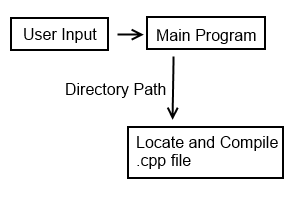
\includegraphics[width=0.75\textwidth]{./DataFlow1}
\end{center}
\caption{Data Flow (Locate and Compile) \label{DataFlow1}}
\end{figure}


\subsection{Design Details}
Here is the code for locating the .cpp file, where root is the full path to the directory the .cpp file is located in:
\begin{lstlisting}
    DIR* dir;
    struct dirent* file;
    std::string filename;
    bool foundFlag = false;
    std::string cppFile;

    dir = opendir( root.c_str() );
    while( ( file = readdir(dir) ) != NULL && !foundFlag )
      {
        //Get the file name
        filename = file -> d_name;
        //skip over "." and ".."
        if( filename != "." && filename != ".." )
          {
        if(filename.find( ".cpp" ) != std::string::npos )
          {
            cppFile = filename;
            foundFlag = true;
          }
          }
      }


    if( !foundFlag )
      {
        std::cout << "Could not find a cpp file." << std::endl;
	std::cout << "Ending Program" << std::endl;
        return 0;
      }
\end{lstlisting}

The following is the code to compile the .cpp file, where root is the directory where the .cpp file is located
and progName is the name of the .cpp file:
\begin{lstlisting}
void Compil(  std::string root, std::string progName )
{
  //Create the argument to send to g++
  std::string progPath = "";
  progPath += root;
  progPath += "/";
  progPath += progName;
  //creat the system command and execute it.
  std::string command;
  command = "g++ " + progPath;
  system( command.c_str() );
 
  return;
}
\end{lstlisting}



\section{Locate the Test Cases }

\subsection{Technologies  Used}
This step of the program relies heavily on the dirent.h library.  It uses a recursive function to search the directory and when
it finds a subdirectory it calls itself to search that subdirectory.

\subsection{Component  Overview}
Two data types from the dirent.h library allow us to search and retrive files from directories.  The first DIR* allows us to open
a specific directory and red from it.  The second struct dirent* is the data type we use to retrive the files we read from a directory.
It has two elements that can be used to categorize the file, d\_name and d\_type.  d\_name is the name of the file, we can use this
to search for certain file extensions, and d\_type is a code for the type of file it is.  This is important in order to find which files are
subdirectories. 

\subsection{Data Flow Diagram}
Figure~\ref{DataFlow2} Shows the Data Flow up to this point.

\begin{figure}[tbh]
\begin{center}
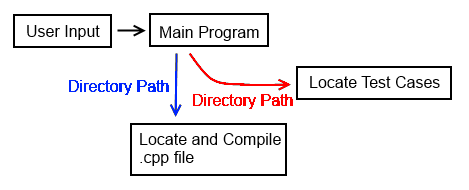
\includegraphics[width=0.75\textwidth]{./DataFlow2}
\end{center}
\caption{Data Flow (Locate and Compile) \label{DataFlow2}}
\end{figure}


\subsection{Design Details}
The following is the function to locate .tst files given a root directory:
\begin{lstlisting}
void DirCrawl( std::string rootDir , std::ofstream &logFile , std::string exec , int &passed , int &tested )
{
	DIR* dir = opendir( rootDir.c_str() );	// Open the directory
	struct dirent* file;	// File entry structure from dirent.h
	std::string filename;	//used in finding if a file has the extention .tst

	// Read each file one at a time
	// Readdir returns next file in the directory, returns null if no other files exist
	while( ( file = readdir(dir)) != NULL )
	{
		//place file name into string filename for easier checking
		filename = file->d_name;

		// skip over the directories "." and ".."
		if ( filename != "." && filename != ".." )
		{
			// checks if the file is a subdirectory, 4 is the integer idetifyer
			// for the dirent struct on Lixux systems
			if ( (int)file->d_type == 4 )
			{
				//moves into the sub-directory
                DirCrawl( rootDir + filename + "/" , logFile , exec , passed , tested );
			}
			else
			{
				// checks if the file has a .tst in it. string find returns
				// string::npos if the substring cannot be found
				if ( filename.find( ".tst") != std::string::npos )
				{
					// pass the file onto the grader 
                    if (run_test_case( rootDir + '/' + filename , exec , logFile ) )
					{
						passed += 1;
					}
					tested += 1;

				}
			}
		}
	}

	closedir(dir);

	return;
}
\end{lstlisting}
The other parameters are passed along to functions it calls, in the case of logFile and exec and passed and tested 
keep track of the number of tests and the number of those that actually passed.


\section{Running a Test Case }

\subsection{Technologies  Used}
This part of the program is done through system calls to the linux terminal. 

\subsection{Component  Overview}
First the program to be tested is run piping the input from the .tst file and the output to a similarly named .out file.
Then using the diff command in linux the .out file, the output of the program, is compared to the .ans file, what should
have been the output of the file.  The console output is piped into a junk file which is later deleted.  If the diff command
returns zero then the files contain the same thing.

\subsection{Data Flow Diagram}
Figure~\ref{DataFlow3} Shows the Data Flow up to this point.

\begin{figure}[tbh]
\begin{center}
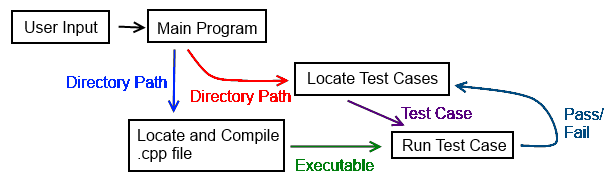
\includegraphics[width=0.75\textwidth]{./DataFlow3}
\end{center}
\caption{Data Flow (Locate and Compile) \label{DataFlow3}}
\end{figure}


\subsection{Design Details}
Here is the function to test an executable with a given test file, it gets passed the logfile to pass it to the function
that writes to the log file.  It returns true if the program passed the test case and false if it did not.
\begin{lstlisting}
bool run_test_case( std::string test_file, std::string exec,
                    std::ofstream &log_file )
{
    std::string out_file = test_file;
    std::string ans_file = test_file;
    std::string test_num = "";
    std::string command_string = "";
    int i;
    int result;

    //get test number
    //name for the test file will be "*case###.tst" so the last number is at
    //position length - 5
    for( i = test_file.length() - 5; test_file[i] >= '0' && test_file[i] <= '9'; i-- )
        //since we are reading in backward the new number gets added at the front
        test_num = test_file[i] + test_num;

    //get text for .out file and .ans file
    //remove tst
    out_file.resize(out_file.size() - 3);
    //add out so we have case#.out
    out_file += "out";

    //remove tst
    ans_file.resize(out_file.size() - 3);
    //add ans so we have case#.ans
    ans_file += "ans";

    //command string = "executable < case.tst > case.out"
    //run the program with input from .tst and pipe output to .out
    command_string = exec + " < " + test_file + " > " + out_file;
    //execute the program
    std::system(command_string.c_str());

    //compare the programs output and the expected output( .out and .ans )
    // diff --ignore-all-space case.out case.ans > nul
    //if it == 0 the files were the same
    // the --ignore ignores whitespace on each line, so trailing spaces
    // or newlines aren't flagged as incorrect
    // > pipes the output into a file called nul
    command_string = "diff --ignore-all-space " + out_file + " " + ans_file + " > nul";
    result = std::system(command_string.c_str());

    //passed test
    if ( result == 0 )
    {
        LogWrite(log_file, test_num,"passed");
        return true;
    }
    //failed test
    else
    {
        LogWrite(log_file, test_num,"failed");
        return false;
    }
}
\end{lstlisting}

\section{Logging the Results}

\subsection{Technologies Used}
The fstream library is used so that we can write to a file.

\subsection{Component Overview}
There are two functions that fall into this, the first is a function that writes out the result of a single test case and the second
writes the final results of the testing.  The ofstream is opened in main to append data so that previous runs on the same
.cpp file are saved.

\subsection{Data Flow Diagram}
Figure~\ref{DataFlow4} Shows the Data Flow up to this point.

\begin{figure}[tbh]
\begin{center}
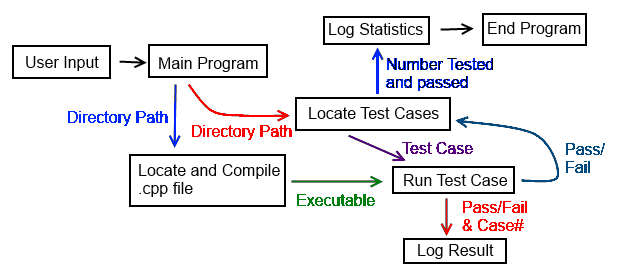
\includegraphics[width=0.75\textwidth]{./DataFlow4}
\end{center}
\caption{Data Flow (Locate and Compile) \label{DataFlow4}}
\end{figure}

\subsection{Design Details}
This first function writes the results of a single test case, it is called by the testing function after it knows determines if the case
passed.
\begin{lstlisting}
void LogWrite( std::ofstream & fout, std::string testNumber, std::string result )
{
  fout << testNumber << ": " << result.c_str() << std::endl;
  return;
  
}
\end{lstlisting}
The second function is called after the directory crawl returns to the main function and writes out the final result of the tests.
\begin{lstlisting}
void FinalLogWrite( std::ofstream & fout, int numPassed, int numTest )
{
  //Calculate the number of tests failed.
  int numFailed;
  numFailed = numTest - numPassed;
  //Calculate the percent passed.
  float perPassed;
  perPassed = (float) numPassed/numTest;
  perPassed =  (int)(perPassed * 100);
  //Calculate the percent failed.
  float perFailed;
  perFailed = (float) numFailed/numTest;
  perFailed = (int)(perFailed * 100);
 
  //Write to stream.
  fout << "Percent of tests Passed: " << perPassed <<  "%" << std::endl;
  fout << "Percent of tests failed: " << perFailed << "%" << std::endl;
  return;
}
\end{lstlisting}



% !TEX root = SystemTemplate.tex

\chapter{System  and Unit Testing}

This section describes the approach taken with regard to system and unit testing. 

\section{Overview}
Provides a brief overview of the testing approach, testing frameworks, and general 
how testing is/will be done to provide a measure of success for the system. 



\section{Dependencies}
Describe the basic dependencies which should include unit testing frameworks and 
reference material. 


\section{Test Setup and Execution}
Describe how test cases were developed, setup, and executed.  This section can 
be extremely involved if a complete list of test cases was warranted for the system. 


% !TEX root = SystemTemplate.tex
\chapter{Development Environment}
Since the program was to test files on a Linux enviornment, it was developed
on a Linux enviornment.


\section{Development IDE and Tools}
No special Tools or IDE were used to develop this.  Since the code was so simple
each programmer just used what ever coding enviornment they wanted.  All
the code was tested on a Linux machine using the g++ compiler.  The debug tool
gdb was used to debug the code when necessary.

\section{Source  Control}
We used github for source control.  The repository can be found at this url: 

https://github.com/TheSoftwareEngineeringAdventureLine/ProgramTesterStage1.git

\section{Dependencies}
This program is dependent on the C++ Standard Library as well as the g++ compiler
on a Linux system.

\section{Build  Environment}
The execuatble is built by the g++ compiler.  You can either compile it manually, using the command:
\begin{lstlisting}
g++ -o tester ProgramTester.cpp
\end{lstlisting}
Or by using the following make file:

\begin{lstlisting}
# compiler
CC = g++

# compiler options
CFLAGS = -c -Wall

all: tester

tester: tester.o
	$(CC) -lm tester.o -o ProgramTester

tester.o: ProgramTester.cpp
	$(CC) $(CFLAGS) ProgramTester.cpp

clean:
	rm -rf *o tester
\end{lstlisting}


% !TEX root = SystemTemplate.tex

\chapter{Release -- Setup -- Deployment}
This section should contain any specific subsection regarding specifics in releasing, 
setup, and/or deployment of the system. 


\section{Deployment Information and Dependencies}
Are there dependencies that are not embedded into the system install? 



\section{Setup Information}
How is a setup/install built? 



\section{System  Versioning Information}
How is the system versioned? 

% !TEX root = SystemTemplate.tex

\chapter{User Documentation}

%This section should contain the basis for any end user documentation for the system. 
 %End user documentation would cover the basic steps for setup and use of the system. 
 %It is likely that the majority of this section would be present in its own document 
%to be delivered to the end user.  However, it is recommended the original is contained 
%and maintained in this document. 

%\newpage   %% 
%%  The user guide can be an external document which is included here if necessary ...
%%  a single source is the way to go.

\section{User Guide}

%The source for the user guide can go here.    You have some options for how to handle the user docs.  If you have some {\tt newpage} commands around the %guide then you can just print out those pages.   If a different formatting is required, then have the source in a separate file {\tt userguide.tex} and include %that file here.  That file can also be included into a driver (like the senior design template) which has the client specified formatting.  Again, this is a single %source approach.   

To use this testing program:
  
 1) make sure that you are in the directory where out program is installed.
 
 2) run the program with on the command line: tester (directory where cpp file and test files are present)
 
 The directory should be the full file path to the proper directory.
 
 Do not put parenthesis around the directory path.
 
 3) the tester program will write a log file to the directory where the cpp file is located.
 
This program is ment to be used with a Linux system.

%% \newpage  %%  if needed ...
\section{Installation Guide}
Insure that ProgramTester.cpp and makefile are in the same
 directory and just type "make" on the command line to install the program
 
 Alternatively you may just compile on the command line with:
 
 g++ ProgramTester.cpp -o tester
  
 Both of these require that you have g++ installed on your system.
 The program is meant to be used on a Linux system.

%% \newpage  %%  if needed ...
\section{Programmer Manual}


% !TEX root = SystemTemplate.tex

\chapter{Class Index}
\section{Class List}
Here are the classes, structs, unions and interfaces with brief descriptions\-:\begin{DoxyCompactList}
\item\contentsline{section}{\hyperlink{class_poly}{Poly} }{\pageref{class_poly}}{}
\end{DoxyCompactList}

\chapter{Class Documentation}
\hypertarget{class_poly}{\section{Poly Class Reference}
\label{class_poly}\index{Poly@{Poly}}
}
\subsection*{Public Member Functions}
\begin{DoxyCompactItemize}
\item 
\hyperlink{class_poly_aa3def076b74bed67904976ad4f9fe9b1}{Poly} ()
\item 
\hyperlink{class_poly_a2f8530284140c31c0aa391dd4d0b61be}{$\sim$\-Poly} ()
\item 
int \hyperlink{class_poly_a14a7ad77ce612b0c54f531d307ee4b39}{myfunction} (int)
\end{DoxyCompactItemize}


\subsection{Constructor \& Destructor Documentation}
\hypertarget{class_poly_aa3def076b74bed67904976ad4f9fe9b1}{\index{Poly@{Poly}!Poly@{Poly}}
\index{Poly@{Poly}!Poly@{Poly}}
\subsubsection[{Poly}]{\setlength{\rightskip}{0pt plus 5cm}Poly\-::\-Poly (
\begin{DoxyParamCaption}
{}
\end{DoxyParamCaption}
)}}\label{class_poly_aa3def076b74bed67904976ad4f9fe9b1}
My constructor \hypertarget{class_poly_a2f8530284140c31c0aa391dd4d0b61be}{\index{Poly@{Poly}!$\sim$\-Poly@{$\sim$\-Poly}}
\index{$\sim$\-Poly@{$\sim$\-Poly}!Poly@{Poly}}
\subsubsection[{$\sim$\-Poly}]{\setlength{\rightskip}{0pt plus 5cm}Poly\-::$\sim$\-Poly (
\begin{DoxyParamCaption}
{}
\end{DoxyParamCaption}
)}}\label{class_poly_a2f8530284140c31c0aa391dd4d0b61be}
My destructor 

\subsection{Member Function Documentation}
\hypertarget{class_poly_a14a7ad77ce612b0c54f531d307ee4b39}{\index{Poly@{Poly}!myfunction@{myfunction}}
\index{myfunction@{myfunction}!Poly@{Poly}}
\subsubsection[{myfunction}]{\setlength{\rightskip}{0pt plus 5cm}int Poly\-::myfunction (
\begin{DoxyParamCaption}
\item[{int}]{a}
\end{DoxyParamCaption}
)}}\label{class_poly_a14a7ad77ce612b0c54f531d307ee4b39}
my own example function fancy new function

new variable 

The documentation for this class was generated from the following file\-:\begin{DoxyCompactItemize}
\item 
hello.\-cpp\end{DoxyCompactItemize}




\backmatter
\chapter{Acknowledgement}
\label{SpecialThanks}  Thanks  


\chapter{Supporting Materials}
This document will contain several appendices used as a way to separate out major 
component details, logic details, or tables of information.  Use of this structure 
will help keep the document clean, readable, and organized. 


%%% Since counters are different in the backmatter section
%%% we explicitly set the section number  (comment out to see effect)
\setcounter{section}{0}
% !TEX root = SystemTemplate.tex

\chapter{Sprint Reports}

\section{Sprint Report \#1}

\section{Sprint Report \#2}

\section{Sprint Report \#3}

% !TEX root = SystemTemplate.tex

\chapter{Industrial Experience}

\section{Resumes}

%    \includepdf[pages={1}]{report.pdf}  %% example of limited page include

%     \includepdf{resume1.pdf}
%     \includepdf{resume2.pdf}
%     \includepdf{resume3.pdf}

\section{Industrial Experience Reports}

\subsection{Name1}

% Report

\subsection{Name2}

% Report

\subsection{Name3}

% Report



\setcounter{section}{0}
% !TEX root = SystemTemplate.tex

\chapter{Appendix}

Latex sample file:  

\section{Introduction}
This is a sample input file.  Comparing it with the output it
generates can show you how to produce a simple document of
your own.

\section{Ordinary Text}  % Produces section heading.  Lower-level
                                    % sections are begun with similar 
                                    % \subsection and \subsubsection commands.

The ends  of words and sentences are marked 
  by   spaces. It  doesn't matter how many 
spaces    you type; one is as good as 100.  The
end of   a line counts as a space.

One   or more   blank lines denote the  end 
of  a paragraph.  

Since any number of consecutive spaces are treated like a single
one, the formatting of the input file makes no difference to
      \TeX,         % The \TeX command generates the TeX logo.
but it makes a difference to you.  
When you use
      \LaTeX,       % The \LaTeX command generates the LaTeX logo.
making your input file as easy to read as possible
will be a great help as you write your document and when you
change it.  This sample file shows how you can add comments to
your own input file.

Because printing is different from typewriting, there are a 
number of things that you have to do differently when preparing 
an input file than if you were just typing the document directly.  
Quotation marks like 
       ``this'' 
have to be handled specially, as do quotes within quotes: 
       ``\,`this'                  % \, separates the double and single quote.
        is what I just 
        wrote, not  `that'\,''.  

Dashes come in three sizes: an 
       intra-word 
dash, a medium dash for number ranges like 
       1--2, 
and a punctuation 
       dash---like 
this.

A sentence-ending space should be larger than the space between words
within a sentence.  You sometimes have to type special commands in
conjunction with punctuation characters to get this right, as in the
following sentence.
       Gnats, gnus, etc.\    % `\ ' makes an inter-word space.
       all begin with G\@.   % \@ marks end-of-sentence punctuation.
You should check the spaces after periods when reading your output to
make sure you haven't forgotten any special cases.
Generating an ellipsis 
       \ldots\    % `\ ' needed because TeX ignores spaces after 
                  % command names like \ldots made from \ + letters.
                  %
                  % Note how a `%' character causes TeX to ignore the 
                  % end of the input line, so these blank lines do not
                  % start a new paragraph.
with the right spacing around the periods 
requires a special  command.  

\TeX\ interprets some common characters as commands, so you must type
special commands to generate them.  These characters include the
following: 
       \$ \& \% \# \{ and \}.

In printing, text is emphasized by using an
       {\em italic\/}  % The \/ command produces the tiny extra space that
                       % should be added between a slanted and a following
                       % unslanted letter.
type style.  

\begin{em}
   A long segment of text can also be emphasized in this way.  Text within
   such a segment given additional emphasis 
          with\/ {\em Roman} 
   type.  Italic type loses its ability to emphasize and become simply
   distracting when used excessively.  
\end{em}

It is sometimes necessary to prevent \TeX\ from breaking a line where
it might otherwise do so.  This may be at a space, as between the
``Mr.'' and ``Jones'' in
       ``Mr.~Jones'',        % ~ produces an unbreakable interword space.
or within a word---especially when the word is a symbol like
       \mbox{\em itemnum\/} 
that makes little sense when hyphenated across 
       lines.

Footnotes\footnote{This is an example of a footnote.}
pose no problem.

\TeX\ is good at typesetting mathematical formulas like
       \( x-3y = 7 \) 
or
       \( a_{1} > x^{2n} / y^{2n} > x' \).
Remember that a letter like
       $x$        % $ ... $  and  \( ... \)  are equivalent
is a formula when it denotes a mathematical symbol, and should
be treated as one.

\section{Displayed Text}

Text is displayed by indenting it from the left margin.
Quotations are commonly displayed.  There are short quotations
\begin{quote}
   This is a short a quotation.  It consists of a 
   single paragraph of text.  There is no paragraph
   indentation.
\end{quote}
and longer ones.
\begin{quotation}
   This is a longer quotation.  It consists of two paragraphs
   of text.  The beginning of each paragraph is indicated
   by an extra indentation.

   This is the second paragarph of the quotation.  It is just
   as dull as the first paragraph.
\end{quotation}
Another frequently-displayed structure is a list.
The following is an example of an {\em itemized} list.
\begin{itemize}
   \item  This is the first item of an itemized list.  Each item 
          in the list is marked with a ``tick''.  The document
          style determines what kind of tick mark is used.

   \item  This is the second item of the list.  It contains another
          list nested inside it.  The inner list is an {\em enumerated}
          list.
          \begin{enumerate}
              \item This is the first item of an enumerated list that
                    is nested within the itemized list.

              \item This is the second item of the inner list.  \LaTeX\
                    allows you to nest lists deeper than you really should.
          \end{enumerate}
          This is the rest of the second item of the outer list.  It
          is no more interesting than any other part of the item.
   \item  This is the third item of the list.
\end{itemize}
You can even display poetry.
\begin{verse}
   There is an environment for verse \\    % The \\ command separates lines
   Whose features some poets will curse.   % within a stanza.

                           % One or more blank lines separate stanzas.

   For instead of making\\
   Them do {\em all\/} line breaking, \\
   It allows them to put too many words on a line when they'd 
   rather be forced to be terse.
\end{verse}

Mathematical formulas may also be displayed.  A displayed formula is
one-line long; multiline formulas require special formatting
instructions.
   \[  x' + y^{2} = z_{i}^{2}\]
Don't start a paragraph with a displayed equation, nor make
one a paragraph by itself.

\section{Build process}

To build \LaTeX\ documents you need the latex program.  It is free and available on all operating systems.   Download and install.  Many of us use the TexLive distribution and are very happy with it.    You can use a editor and command line or use an IDE.  To build this document via command line:

\begin{verbatim}
alta>  pdflatex SystemTemplate
\end{verbatim}
If you change the bib entries, then you need to update the bib files:
\begin{verbatim}
alta>  pdflatex SystemTemplate
alta>  bibtex SystemTemplate
alta>  pdflatex SystemTemplate
alta>  pdflatex SystemTemplate
\end{verbatim}


\section*{Acknowledgement}
Thanks to Leslie Lamport





\bibliography{designrefs.bib}
\bibliographystyle{plain}



\end{document}
